\documentclass[aspectratio=169,11pt]{beamer}
\usepackage[T1]{fontenc}
\usepackage{helvet}
\usepackage{amsmath}
\usepackage{booktabs}
\usepackage{tikz}
\usetikzlibrary{arrows.meta,positioning}

% ── minimal clean theme ─────────────────────────────────────────────
\usetheme{default}
\setbeamertemplate{navigation symbols}{}
\setbeamertemplate{footline}[frame number]
\definecolor{cblue}{HTML}{2a78d6}
\definecolor{corange}{HTML}{eb6834}
\definecolor{caqua}{HTML}{1baf7a}
\definecolor{cgray}{HTML}{6b6a66}
\setbeamercolor{frametitle}{fg=cblue}
\setbeamercolor{title}{fg=cblue}
\setbeamercolor{structure}{fg=cblue}
\setbeamerfont{frametitle}{series=\bfseries,size=\large}
\setbeamertemplate{blocks}[rounded]
\setbeamercolor{block title}{bg=cblue!12,fg=cblue}
\setbeamercolor{block body}{bg=cblue!4,fg=black}
\setbeamercolor{block title alerted}{bg=corange!15,fg=corange}
\setbeamercolor{block body alerted}{bg=corange!4,fg=black}
\newcommand{\good}[1]{\textcolor{caqua}{#1}}
\newcommand{\bad}[1]{\textcolor{corange}{#1}}
\graphicspath{{../figs/}}

\title{The $^{27}$Al(n,$\gamma$) capture rate on the He-3 capsule:\\
       an analytic cross-check of Geant4}
\author{Claude (Fable~5) for Dylan \\ MX17 / nTOF EAR2}
\date{2026-07-23}

\begin{document}

\begin{frame}
  \titlepage
  \vspace{-1.2em}
  \centering
  \footnotesize\color{cgray}
  Task: \texttt{.claude/al\_gamma\_yield\_check/HANDOFF.md} ---
  is the Geant4 Al-capture background rate right, and why did a
  back-of-envelope estimate look low?
\end{frame}

% ────────────────────────────────────────────────────────────────────
\begin{frame}{The question}
  \begin{columns}[T]
    \column{0.58\textwidth}
    \textbf{Geant4 says} the Al pressure vessel of the He-3 capsule glows:
    \begin{itemize}
      \item $5.95\times10^{6}$ $\gamma\!\to\!e^{+}e^{-}$ pairs/day produced
            from the 7.72\,MeV Al(n,$\gamma$) line --- the dominant e$^+$e$^-$
            background to the X17 search.
    \end{itemize}
    \medskip
    \textbf{A hand calculation} (13\,g Al, single-pass slab,
    beam below 1\,eV) gave a $\gamma$ yield that \emph{looked low}.
    \medskip

    \textbf{This cross-check} compares at the cleanest level:
    \emph{radiative captures in the Al}, before any pair-conversion folding.
    \column{0.40\textwidth}
    \begin{block}{\small Comparison quantity}
      \small
      EventTree, 20 files $\times$ $10^{7}$ thermal neutrons
      ($E\in[1\,\text{meV},2\,\text{eV}]$):
      \smallskip

      \texttt{capture\_vol == He3Cap\_Al}\\
      \texttt{capture\_proc == nCapture}
      \smallskip

      $1{,}561{,}193$ captures $/\,2\times10^{8}$ n\\
      $= 7.81\times10^{-3}$ per neutron\quad($\pm$0.08\%)
    \end{block}
  \end{columns}
\end{frame}

% ────────────────────────────────────────────────────────────────────
\begin{frame}{First finding: the capsule faces the beam valve-first}
  \centering
  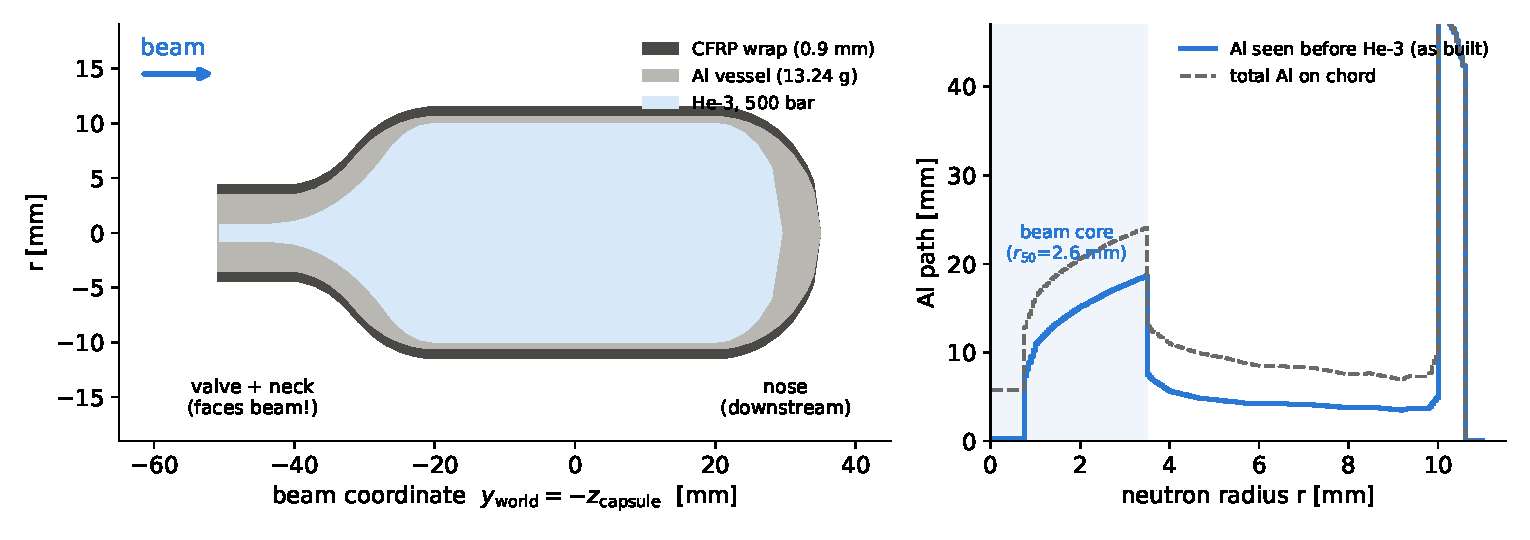
\includegraphics[width=0.9\textwidth]{geometry.pdf}

  \begin{columns}[T]
    \column{0.55\textwidth}
    \small
    The placement rotation (\texttt{rotateX(-90$^\circ$)}) maps local
    $z \to -y_{\rm world}$: the \textbf{valve} (local $z=+51$\,mm) sits at
    $y=-51$\,mm, \emph{upstream}, facing the gun.
    \column{0.42\textwidth}
    \small
    The beam core ($r_{50}=2.6$\,mm) bores through the nearly solid Al
    valve stem + shoulder: \textbf{10--20\,mm of Al}, not 5.5\,mm of nose,
    not 0.6\,mm of wall.
  \end{columns}
\end{frame}

% ────────────────────────────────────────────────────────────────────
\begin{frame}{How we know the orientation (it's in the data)}
  \begin{columns}[T]
    \column{0.5\textwidth}
    \small
    Geant4 records the capture position per event
    (\texttt{cap\_x,y,z}). Where the Al captures actually happen:
    \medskip

    \begin{tabular}{lr}
      \toprule
      capsule region & captures \\
      \midrule
      valve stem ($z\!\in\![40,51]$) & \textbf{68.3\%} \\
      shoulder taper ($z\!\in\![21,40]$) & 28.5\% \\
      barrel wall ($|z|<21$) & 3.0\% \\
      nose dome ($z<-21$) & \textbf{0.2\%} \\
      \bottomrule
    \end{tabular}
    \medskip

    96.6\% of captures at $r<10$\,mm --- the valve/neck, not the barrel wall.
    \column{0.48\textwidth}
    \small
    \begin{alertblock}{\small If the nose faced the beam}
      the nose would capture first and the valve would hide behind
      17\,cm$^{3}$ of black He-3. Instead the nose is \emph{empty} and the
      valve \emph{saturated}: the valve faces the beam.
    \end{alertblock}
    \smallskip
    \begin{block}{\small Why it matters}
      He-3 at 500\,bar is optically thick ($\lambda_{\rm abs}\approx25\,\mu$m
      at 25\,meV): whatever Al lies \emph{behind} first gas contact is
      invisible. Orientation alone changes the capture rate by
      $\times 1.8$.
    \end{block}
  \end{columns}
\end{frame}

% ────────────────────────────────────────────────────────────────────
\begin{frame}{Ingredients of the analytic model}
  \begin{columns}[T]
    \column{0.52\textwidth}
    \textbf{Beam} (exactly as the sim samples it)
    \begin{itemize}\small
      \item energy: EAR2 flux histogram,
            $\Phi = 4.29\times10^{6}$\,n/pulse in [1\,meV, 2\,eV]
            ($3.99\times10^{6}$ below 1\,eV)
      \item radius: \texttt{Lambda2D} profile row nearest in $\log E$
            ($r_{50}=2.6$\,mm, $r_{90}=13$\,mm; 86\% inside the capsule face)
      \item $1.929\times10^{4}$ pulses/day
    \end{itemize}
    \smallskip
    \textbf{Geometry}: exact STEP polycones, mirrored from
    \texttt{DetectorConstruction.cc}; reproduces
    $V_{\rm Al}=4.907$\,cm$^{3}$, $V_{\rm gas}=17.003$\,cm$^{3}$ to 4 digits.
    \column{0.46\textwidth}
    \textbf{Nuclear data} (ENDF / IAEA EGAF)
    \begin{itemize}\small
      \item $^{27}$Al(n,$\gamma$): $\sigma_{0}=0.231$\,b at 25.3\,meV,
            $1/v$ below the 5.9\,keV resonance
      \item cross-check: the $^{28}$Al $\beta$-decay line (1778.9\,keV,
            $\sim$1 per capture) has $\sigma_{\gamma}=0.232(4)$\,b \good{\checkmark}
      \item \textbf{7724\,keV line: $\sigma_{\gamma}=0.0493(15)$\,b
            $\Rightarrow$ 21.3\% of captures} (not 1 per capture!)
      \item $^{3}$He(n,p)t: ENDF (5333\,b at 25.3\,meV, $1/v$)
      \item Al elastic $\approx$1.4\,b (6$\times$ capture: ignored in
            single-pass, checked against Geant4)
    \end{itemize}
  \end{columns}
\end{frame}

% ────────────────────────────────────────────────────────────────────
\begin{frame}{Method: single-pass straight-line attenuation}
  \begin{block}{}
    \vspace{-1.5em}
    \begin{align*}
      R \;=\; \sum_{E\,\rm bins} \Phi(E) \int \!f(r|E)\,dr
      \underbrace{\int_{\rm path}\! dz\;
      \Sigma_{\gamma}^{\rm Al}(E)\,\mathbb{1}_{\rm Al}(r,z)\;
      e^{-\Sigma_{\gamma}^{\rm Al} t_{\rm Al}(z) \,-\,
         \Sigma_{\rm abs}^{\rm He3} t_{\rm gas}(z)}}_{\text{capture prob.\ on the straight chord at radius } r}
    \end{align*}
    \vspace{-1.2em}
  \end{block}
  \small
  \begin{columns}[T]
    \column{0.5\textwidth}
    \textbf{Includes}
    \begin{itemize}
      \item exact thickness-vs-radius profile (0.02\,mm marching)
      \item He-3 shadowing with the true $\sigma(E)$ (the gas is black
            below $\sim$1\,keV)
      \item $1/v$ folded over the real flux spectrum, bin by bin
      \item the same radial-profile-vs-energy correlation the gun uses
    \end{itemize}
    \column{0.47\textwidth}
    \textbf{Deliberately ignores} (checked a posteriori)
    \begin{itemize}
      \item elastic scattering in Al/CFRP/air (redirects, $\sim$6:1 over
            capture)
      \item albedo from the surrounding plastics/LS
      \item these partially cancel: out-scatter $-$, re-entry $+$
    \end{itemize}
  \end{columns}
\end{frame}

% ────────────────────────────────────────────────────────────────────
\begin{frame}{Result: the ladder from ``thin disk'' to truth}
  \centering
  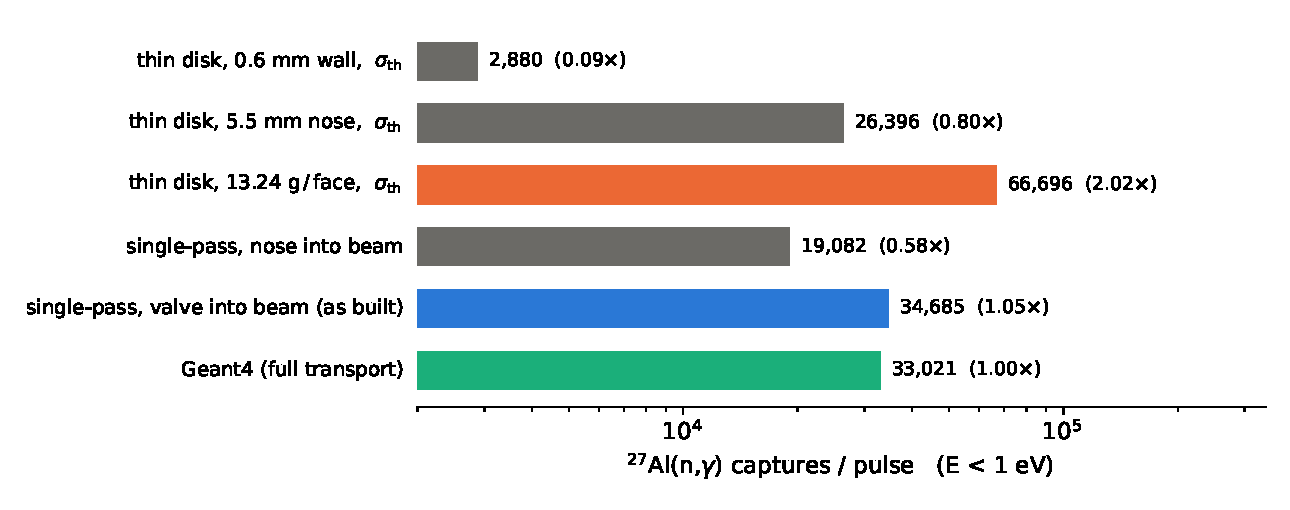
\includegraphics[width=0.86\textwidth]{buildup.pdf}

  \small
  \bad{Wall-slab: 11$\times$ low.} \bad{Mass-smeared: 2$\times$ high.}
  \good{Single-pass on the true geometry: within 5\% of Geant4.}
\end{frame}

% ────────────────────────────────────────────────────────────────────
\begin{frame}{The capture map: the model predicts \emph{where}, too}
  \centering
  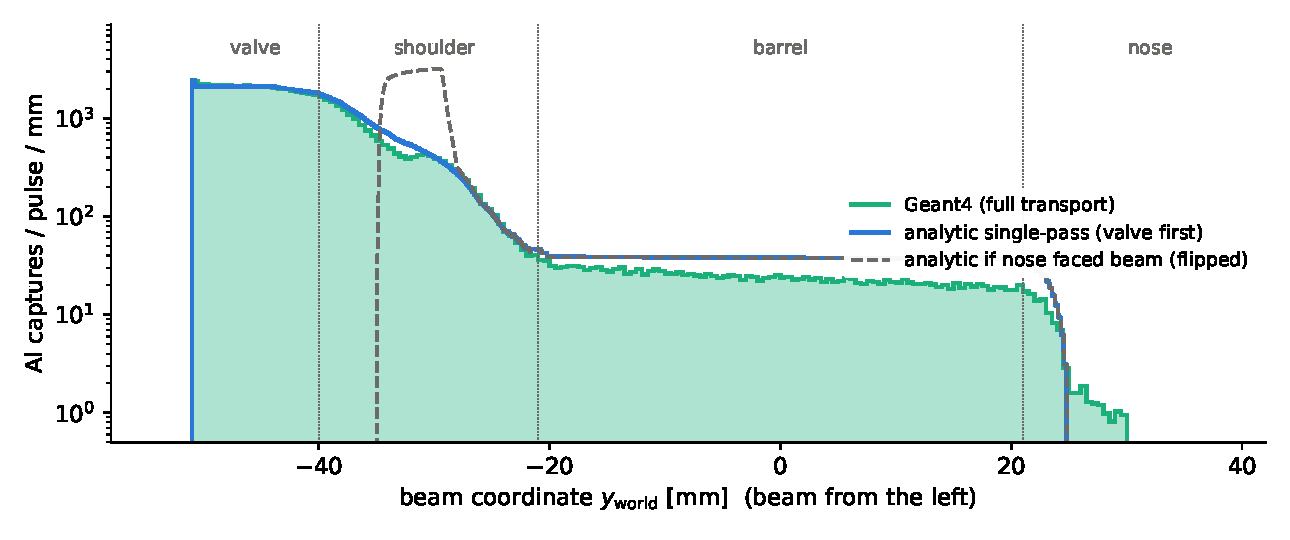
\includegraphics[width=0.88\textwidth]{axial_profile.pdf}
  \vspace{-0.4em}
  \small

  Geant4 and the straight-line model agree over three decades along the
  capsule. The counterfactual flipped mounting (dashed) would capture
  $1.8\times$ less, concentrated in the nose dome.
\end{frame}

% ────────────────────────────────────────────────────────────────────
\begin{frame}{Same story in 2D and in energy}
  \centering
  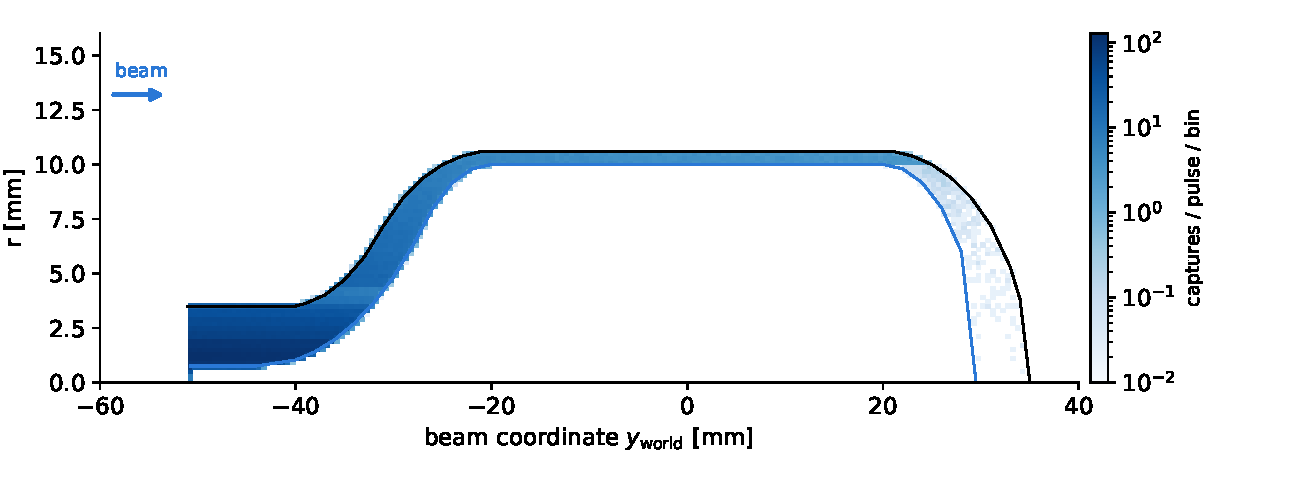
\includegraphics[width=0.75\textwidth]{capture_map.pdf}
  \vspace{-0.5em}
  \small

  Captures hug the upstream Al surfaces (Geant4; outlines: Al black,
  gas blue). The energy spectrum of capturing neutrons matches shape-wise
  with a flat $\sim$0.95 ratio (backup slide).
\end{frame}

% ────────────────────────────────────────────────────────────────────
\begin{frame}{What the thin-disk assumptions cost --- ranked}
  \small
  \begin{tabular}{p{5.6cm}cp{5.2cm}}
    \toprule
    effect & factor & comment \\
    \midrule
    \textbf{which Al the beam sees} & & the dominant issue \\
    \quad 0.6\,mm wall slab & \bad{$\times$0.09} & beam core never sees the wall \\
    \quad 5.5\,mm nose slab & $\times$0.8 & fortuitously close, wrong picture \\
    \quad 13.24\,g smeared over the face & \bad{$\times$2.0} & counts shadowed Al
          (3.7\,g behind gas) and ignores where flux is \\
    \quad orientation (valve vs nose first) & \bad{$\times$1.8} & as-built:
          valve first, $\langle t_{\rm pre}\rangle = 9.1$\,mm \\
    \midrule
    $\sigma_{\rm th}$ instead of
    $\langle\sigma\rangle_{\rm flux}$ & \bad{$\times$1.45} & the $<$1\,eV window
          is \emph{above} 25\,meV on average; sub-thermal $1/v$ gain never
          compensates \\
    \midrule
    straight line vs full transport & \good{$\times$0.95} & scattering out
          $\approx$ albedo in; He-3 absorbs 77\% (G4) vs 91\% (straight line) \\
    \midrule
    assuming 1\,$\gamma$(7.72\,MeV)/capture & \bad{$\times$4.7} & EGAF: 21.3\%
          of captures \\
    \bottomrule
  \end{tabular}
\end{frame}

% ────────────────────────────────────────────────────────────────────
\begin{frame}{The quotable one-line calculation}
  \begin{block}{}
    \centering
    $R \;=\; \Phi \times n_{\rm Al}\,\bar\sigma_{\gamma} \times
    \langle t_{\rm pre}\rangle
    \;=\; 4.29\times10^{6} \times \left(6.02\times10^{22}\,\tfrac{1}{\rm cm^{3}}
    \times 0.150\,{\rm b}\right) \times 9.1\,{\rm mm}
    \;\approx\; 3.5\times10^{4}\ \text{captures/pulse}$
  \end{block}
  \small
  \begin{itemize}
    \item $\bar\sigma_{\gamma} = 0.231\,\text{b} \times 0.65$: thermal
          cross-section folded with the actual [1\,meV, 2\,eV] spectrum ($1/v$)
    \item $\langle t_{\rm pre}\rangle = 9.1$\,mm: flux-weighted Al path
          \emph{before first He-3 contact} (valve-first); the only nontrivial
          geometry number
    \item optically thin ($\Sigma_\gamma \langle t\rangle \approx 0.8\%$), so
          everything factorizes
  \end{itemize}
  \medskip
  \centering
  \begin{tabular}{lccc}
    \toprule
    $[1\,\text{meV},2\,\text{eV}]$ & per pulse & per day & vs Geant4 \\
    \midrule
    one-line / full single-pass & $35{,}180$ & $6.79\times10^{8}$ & $+5\%$ \\
    \textbf{Geant4} & $\mathbf{33{,}508}$ & $\mathbf{6.46\times10^{8}}$ & --- \\
    \bottomrule
  \end{tabular}
\end{frame}

% ────────────────────────────────────────────────────────────────────
\begin{frame}{From captures to the 7.72\,MeV $\gamma$ (and to pairs)}
  \small
  \begin{columns}[T]
    \column{0.55\textwidth}
    \begin{tabular}{lcc}
      \toprule
      (Geant4-anchored) & per pulse & per day \\
      \midrule
      Al captures, $E_n\!<\!2$\,eV & $33{,}508$ & $6.5\times10^{8}$ \\
      $\gamma$(7.724\,MeV), 21.3\% & $7{,}151$ & $1.4\times10^{8}$ \\
      $\gamma\!\to\!e^{+}e^{-}$ anywhere & $\sim$328 & $6.4\times10^{6}$ \\
      \quad (of which in Al) & 308 & $6.0\times10^{6}$ \\
      \bottomrule
    \end{tabular}
    \smallskip

    Extending to $E_n<1$\,keV adds only \textbf{+3.6\%} captures
    (analytic): $\Phi$ grows 1.7$\times$ but $\sigma\!\sim\!1/v$ dies.
    \column{0.43\textwidth}
    \begin{itemize}
      \item pair conversion of the 7.72\,MeV line costs another
            $\sim$2\% (from the sim's own conv-pair campaign) ---
            \emph{that} chain, not the capture rate, is where the small
            numbers come from
      \item if a hand calc also used 1\,$\gamma$/capture and the 0.6\,mm
            wall, errors of $\times4.7$ (up) and $\times11$ (down) fight:
            ``looks low'' is the expected outcome
    \end{itemize}
  \end{columns}
\end{frame}

% ────────────────────────────────────────────────────────────────────
\begin{frame}{Conclusions}
  \begin{enumerate}
    \item \good{\textbf{The Geant4 number is right.}} An independent
          straight-line calculation on the true geometry reproduces the
          capture rate to \textbf{+5\%} and the capture \emph{locations}
          and \emph{energy spectrum} in detail. Nothing about the
          $6\times10^{8}$ captures/day ($1.4\times10^{8}$
          7.72\,MeV\,$\gamma$/day) is anomalous.
    \item \textbf{Thin-disk is inadequate here} unless ``thickness'' means
          the flux-weighted pre-gas Al path (9.1\,mm). Wall/nose/mass
          variants land anywhere from $0.09\times$ to $2\times$.
    \item The two knobs that matter beyond geometry:
          $\langle\sigma\rangle/\sigma_{\rm th}=0.65$ (window average) and
          21.3\% for the 7.724\,MeV line.
    \item \bad{\textbf{Action item: confirm the capsule mounting.}}
          The sim as built has the \emph{valve facing the beam}; the handoff
          (and probably our mental model) assumed nose-first. If the real
          mounting is nose-first, the Al capture background drops
          $\times0.55$ --- and the sim placement (\texttt{rotateX}) needs a
          sign fix, re-running the Al-pair background chain.
  \end{enumerate}
\end{frame}

% ════════════════════════════════════════════════════════════════════
%  PART II — from gammas to single-arm coincidences
% ════════════════════════════════════════════════════════════════════
\begin{frame}{Part II: from $\gamma$s to single-arm coincidences}
  \small
  \textbf{Alberto's calculation} (email 2026-07-23) vs this work, per pulse:
  \medskip

  \centering
  \begin{tabular}{lccc}
    \toprule
    & Alberto & this work (G4) & ratio \\
    \midrule
    Al captures, $E_n<1$\,eV & 72{,}787 & 33{,}021 & 2.2 \\
    \quad model & 13\,g thin disk, $r\!\approx\!1$\,cm & full transport & \\
    7.72\,MeV $\gamma$ intensity & 26.8\,\% & 21.3\,\% (EGAF) & 1.26 \\
    $\gamma_0$ produced, $E_n<1$\,eV & 19{,}507 & 7{,}033 & 2.8 \\
    $\gamma_0$ into detector & 878 ($\Omega$=4.5\,\%) & see next slide & \\
    \textbf{single-arm coincidences} & $\sim$9 ($\times$1\,\%) & \textbf{199} & \bad{$\sim$22} \\
    \bottomrule
  \end{tabular}
  \medskip

  \raggedright
  The capture/$\gamma$ level \good{agrees to a understood factor $\sim$2}
  (his thin disk = the ``mass-smeared'' rung of our ladder; bin-by-bin ratio
  2.2--2.4 below 1\,eV, same spectral shape). The \bad{$\times$22 tension} is
  entirely downstream of the $\gamma$ yield.
\end{frame}

% ────────────────────────────────────────────────────────────────────
\begin{frame}{What the sim counts: ``legs'' (SiPM $\wedge$ plastic per arm)}
  \small
  \begin{columns}[T]
    \column{0.55\textwidth}
    Per arm: $S$ = max single SiPM-bar edep, $P$ = max plastic-bar edep;
    leg $\equiv S\geq0.5$\,MIP $\wedge$ $P\geq0.5$\,MIP, in-gate ($>$1\,ms).
    \medskip

    \begin{tabular}{lcc}
      \toprule
      legs/pulse (arm-summed) & 2.0 cm & 2.5 cm \\
      \midrule
      baseline & 203.4 & 168.5 \\
      no-Al capsule & 4.6 & 3.3 \\
      \textbf{Al-attributable} & \textbf{198.8} & 165.2 \\
      \bottomrule
    \end{tabular}
    \smallskip

    $\approx$\,\textbf{50 legs/arm/pulse} --- Dylan's number \good{\checkmark}
    \column{0.43\textwidth}
    Thresholds in energy:
    \begin{itemize}
      \item SiPM bar (3\,mm PVT): 0.5\,MIP = \textbf{0.23\,MeV}
      \item plastic (2.0\,cm PVT): 0.5\,MIP = \textbf{1.73\,MeV}
            (the 1.78\,MeV $^{28}$Al decay line is delayed 2.2\,min
            \emph{and} below max-Compton threshold --- irrelevant)
    \end{itemize}
  \end{columns}
\end{frame}

% ────────────────────────────────────────────────────────────────────
\begin{frame}{Apertures: Alberto's 4.5\,\% is ONE arm of four}
  \small
  From the capture centroid (valve, $y\simeq-4.5$\,cm):
  \medskip

  \centering
  \begin{tabular}{lcccc}
    \toprule
    surface & size & distance & $\Omega/4\pi$ per arm & $\times$4 arms \\
    \midrule
    SiPM wall (3\,mm) & 40$\times$50\,cm & 33.2\,cm & 10.1\,\% & \textbf{40.3\,\%} \\
    plastics (2\,cm) & 40.3$\times$30\,cm & $\sim$42\,cm & \textbf{4.6\,\%} & \textbf{18.5\,\%} \\
    \bottomrule
  \end{tabular}
  \medskip

  \raggedright
  Alberto's ``solid angle covered = 4.5\,\%'' equals one arm's plastic
  aperture almost exactly. The coincidence-limiting aperture (plastics,
  4 arms) is \bad{$\times$4.1 larger}; the SiPM wall sees $\times$9 his
  solid angle.
\end{frame}

% ────────────────────────────────────────────────────────────────────
\begin{frame}{Scintillator material is NOT the explanation ($\pm$10\,\%)}
  \small
  Compton is electron-density physics; every CH-based plastic is the same to
  $\pm$10\,\%. Klein--Nishina interaction probabilities:
  \medskip

  \centering
  \begin{tabular}{lccc}
    \toprule
    material & $n_e$ [$10^{23}$/cm$^3$] & $P_C$(2\,cm, 7.72\,MeV) & $P_C$(2\,cm, 3.03\,MeV) \\
    \midrule
    PVT (EJ-200 family; sim) & 3.37 & 4.05\,\% & 7.40\,\% \\
    polystyrene-based & 3.40 & 4.09\,\% & 7.48\,\% \\
    PMMA (acrylic) & 3.87 & 4.64\,\% & 8.46\,\% \\
    polyethylene & 3.23 & 3.89\,\% & 7.11\,\% \\
    \bottomrule
  \end{tabular}
  \medskip

  \raggedright
  Pair production adds $\sim$0.9\,\% at 7.72\,MeV (2\,cm). The 3\,mm SiPM bar
  has $P_C=0.62\,\%$ at 7.72\,MeV --- \textbf{Alberto's ``$\sim$1\,\%
  Compton'' describes the thin SiPM bar, not the 2\,cm plastic (4--5\,\%,
  and 7--8\,\% for the 3--4.7\,MeV cascade lines).}
\end{frame}

% ────────────────────────────────────────────────────────────────────
\begin{frame}{Geant4's answer: ONE electron makes both signals}
  \small
  Two truth runs: every leg classified in $6\times10^{7}$ neutron events
  (2{,}868 legs, real cascade), and a dedicated \textbf{$\gamma$-source truth
  run} ($4\times10^{6}$ single cascade $\gamma$s from real capture vertices,
  11{,}181 legs, with birth volume/process recorded per track):
  \medskip

  \begin{columns}[T]
    \column{0.5\textwidth}
    {\scriptsize\setlength{\tabcolsep}{4pt}
    \begin{tabular}{lr}
      \toprule
      leg mechanism (combined truth) & fraction \\
      \midrule
      \textbf{one track crosses bar+plastic} & \textbf{98\,\%} \\
      \quad via hard Compton & 80.0\,\% \\
      \quad via pair production & 17.9\,\% \\
      \quad birth KE (median) & 4.5 MeV \\
      same $\gamma$, two interactions & 0.4\,\% \\
      two different cascade $\gamma$s & 1.2\,\% \\
      \midrule
      crossing track also crossed the MM & \textbf{52\,\%} \\
      \bottomrule
    \end{tabular}}
    \column{0.47\textwidth}
    \begin{alertblock}{\small The broken assumption}
      A coincidence does NOT cost $P_{\rm SiPM}\times P_{\rm plastic}$ ---
      one interaction anywhere upstream buys both signals: the multi-MeV
      electron crosses the 3\,mm bar (0.23\,MeV) and buries itself in the
      2\,cm plastic (1.73\,MeV). Measured response to an emitted 7.72\,MeV
      $\gamma$: \textbf{0.54\,\%} (all arms) = 2.9\,\% per $\gamma$ through
      the plastic aperture.
    \end{alertblock}
    \smallskip
    Half the leg electrons are born at the \emph{capsule} and fly
    $\sim$33\,cm through the MM --- they leave an MM track (veto handle!).
  \end{columns}
\end{frame}

% ────────────────────────────────────────────────────────────────────
\begin{frame}{The four ways a leg happens --- with measured fractions}
  \centering
  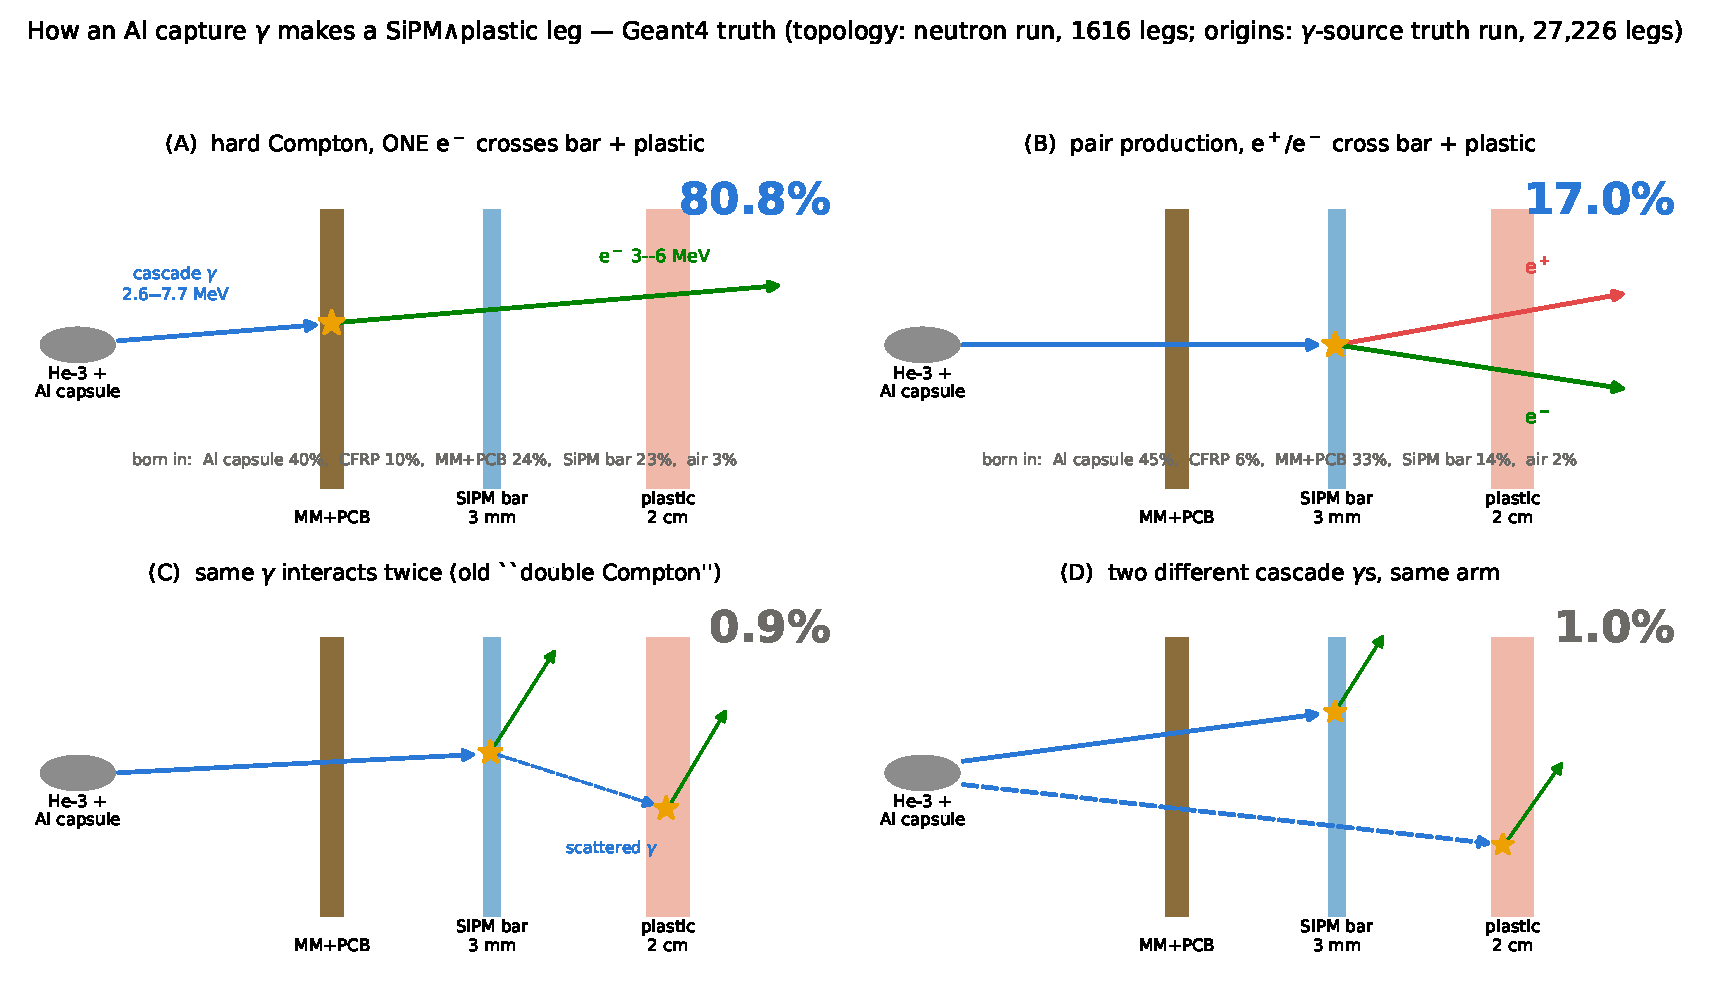
\includegraphics[width=0.98\textwidth]{leg_mechanism_corrected.pdf}
\end{frame}

% ────────────────────────────────────────────────────────────────────
\begin{frame}{Where the leg-making electron is born, and which line sent it}
  \centering
  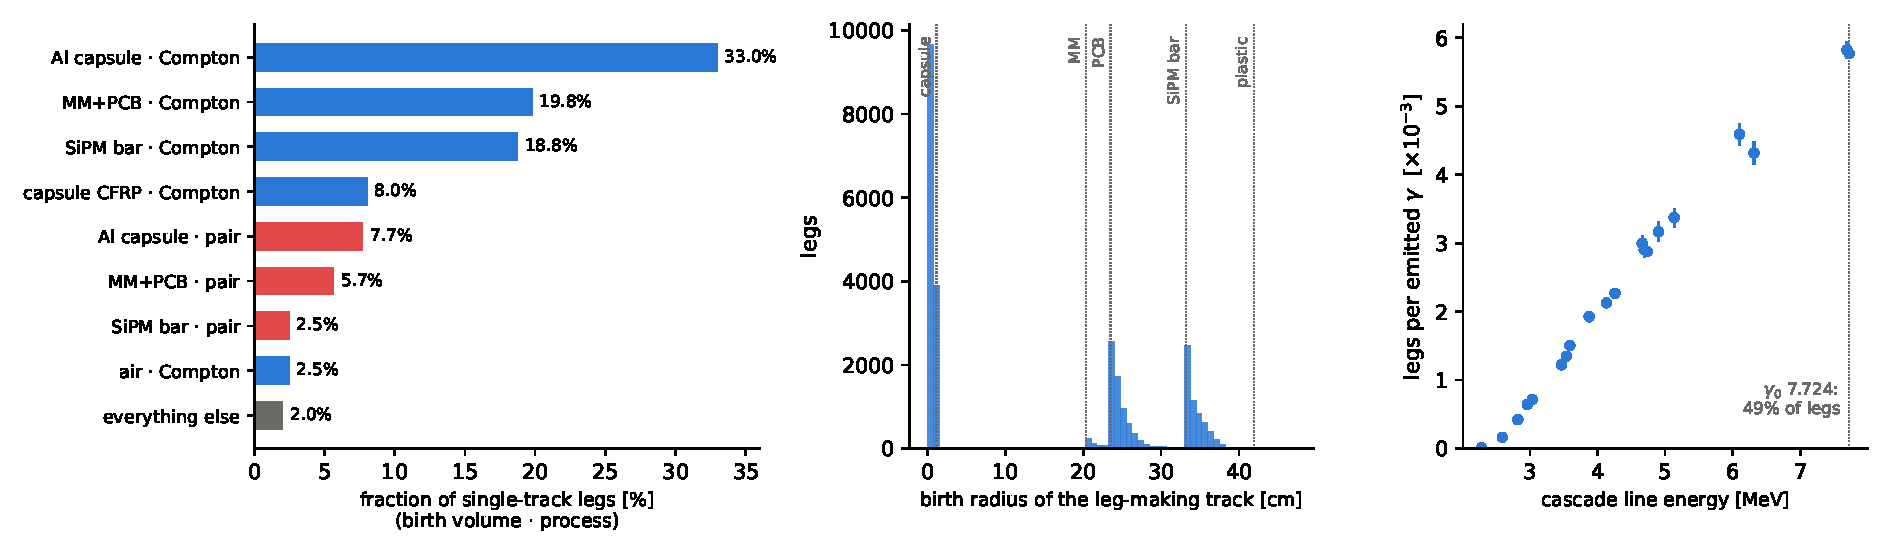
\includegraphics[width=\textwidth]{leg_origin_breakdown.pdf}

  \small\raggedright
  Left: birth volume $\times$ process (Compton blue, pair red). Middle: birth
  radius --- the capsule itself is the single biggest electron source, then
  the MM PCB and the SiPM bar; essentially nothing starts in the plastic.
  Right: legs per emitted $\gamma$ vs line energy --- zero below 2.3\,MeV
  (plastic threshold), rising steeply; the 7.724\,MeV line alone makes
  \textbf{47\,\% of all legs}.
\end{frame}

% ────────────────────────────────────────────────────────────────────
\begin{frame}{The reconciliation ladder: 9 $\to$ 199 legs/pulse}
  \centering
  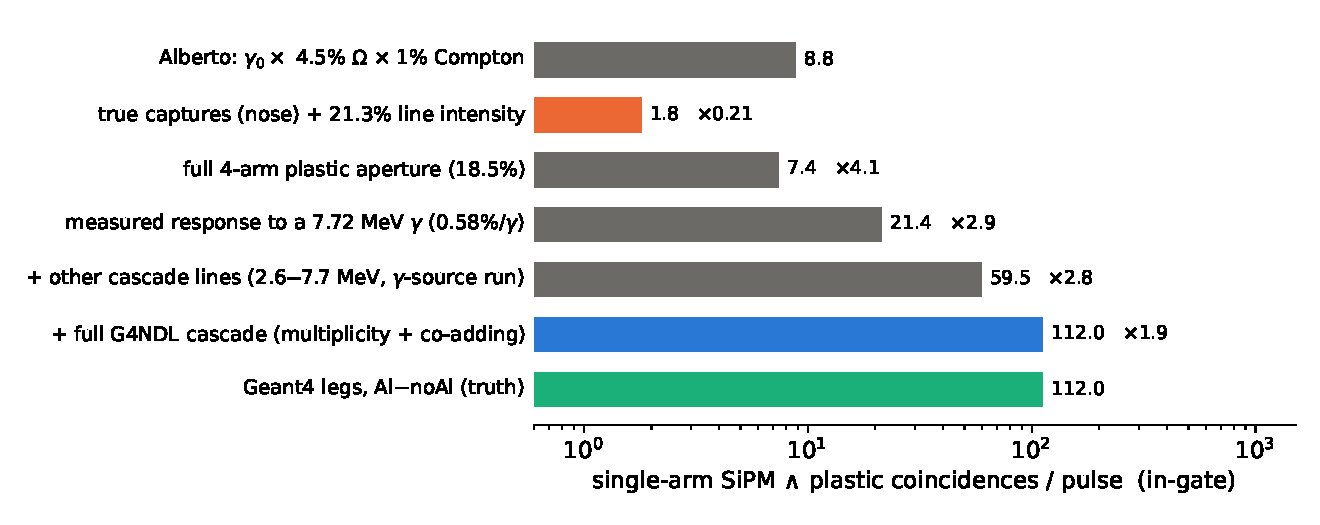
\includegraphics[width=0.94\textwidth]{coincidence_ladder.pdf}

  \small
  \raggedright
  Every rung is now \emph{measured}: the 7.72-$\gamma$ response
  (0.54\,\%/emitted $\gamma$) and the cascade-line sum come from the
  $\gamma$-source truth run; the last rung ($\times$1.9) is the full G4NDL
  cascade vs the 20-line discrete list (multiplicity/continuum +
  within-cascade co-adding). No single error --- five compounding
  assumptions. The scintillator \emph{material} is irrelevant
  ($\pm$10\,\%).
\end{frame}

% ────────────────────────────────────────────────────────────────────
\begin{frame}{Orientation history: it was never flipped --- it was born this way}
  \small
  \begin{description}
    \item[2026-06-01] \texttt{rotateX(-90$^\circ$)} + beam $+Y$ introduced ---
      capsule still a symmetric cylinder (\texttt{G4Tubs}); orientation
      meaningless.
    \item[2026-06-10] STEP polycone lands (tip $z=-35$, valve $+51$) under the
      \emph{pre-existing} rotation $\Rightarrow$ \bad{valve-upstream from day
      one}.
    \item[2026-06-11] thermal\_note: prose says beam ``enters through a
      5\,mm-thick domed aluminium tip'' (the intention), but its own quoted
      rate --- \textbf{capture in Al capsule $8.0\times10^{-3}$} --- is the
      \emph{valve-first} number (nose-first $=4.5\times10^{-3}$). The sim was
      already flipped then.
    \item[06-30 / 07-14 / 07-15] axis convention, MM spacing, stack flip:
      none touch \texttt{capRot} or the polycone $z$ arrays (verified by
      diff).
    \item[2026-07-22] event display draws $y_{\rm world}=-z_{\rm local}$
      (correct, valve upstream).
  \end{description}
  \medskip
  \good{Silver lining:} every thermal-era result is internally consistent ---
  all valve-first.
\end{frame}

% ────────────────────────────────────────────────────────────────────
\begin{frame}{Conclusions --- Part II}
  \begin{enumerate}
    \item \good{\textbf{The sim's $\sim$50 legs/arm/pulse (199 summed) is
          right}} --- and Alberto's 9/pulse is right \emph{for his
          assumptions}. The gap: four-arm aperture ($\times$4.1), the real
          response to a 7.72\,$\gamma$ ($\times$2.9 --- a \emph{single}
          3--6\,MeV Compton/pair electron crosses both detectors, 80/18\,\%),
          the rest of the cascade ($\times$2.8), and the full-cascade
          correction ($\times$1.9). Half the leg electrons are born at the
          capsule and cross the MM $\Rightarrow$ an MM-track veto could kill
          $\sim$50\,\% of trigger legs.
    \item \textbf{The plastic material is not the variable}: every CH-based
          scintillator is within $\pm$10\,\% (electron-density physics).
          The thicknesses and the upstream material (MM PCB, container,
          bar) are what matter.
    \item Capture/$\gamma$-yield level: we and Alberto agree once his thin
          disk is corrected by the known $\times$2.2 (geometry + shadowing
          + $\sigma$ folding) and 26.8\,\% $\to$ 21.3\,\% (EGAF).
    \item Orientation: valve-first since the STEP capsule existed
          (2026-06-10); nothing was flipped by the axis change. All
          thermal-era numbers are internally consistent. \bad{Still open:
          which way is the \emph{real} capsule mounted?} (nose-first
          $\Rightarrow$ captures $\times$0.55, and the capture zone moves
          14\,cm downstream --- leg rates would change too.)
  \end{enumerate}
\end{frame}

% ────────────────────────────────────────────────────────────────────
\begin{frame}{Backup: energy spectrum of capturing neutrons}
  \centering
  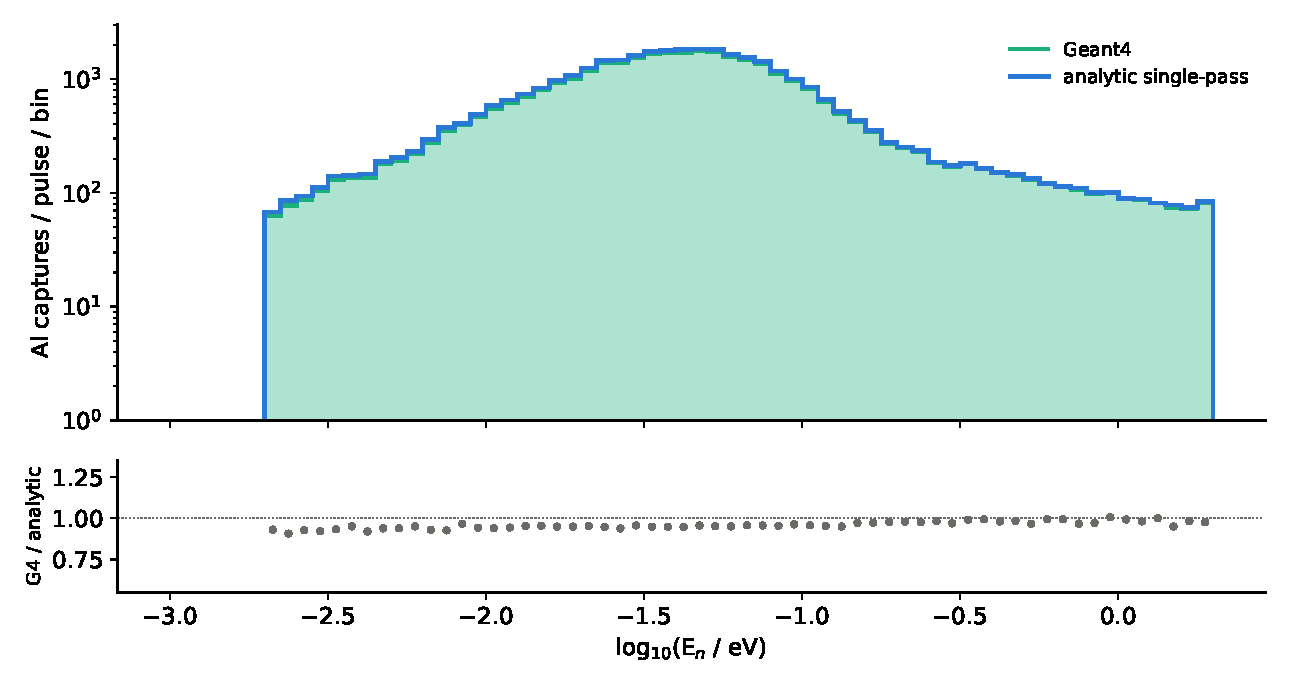
\includegraphics[width=0.8\textwidth]{espec.pdf}
\end{frame}

\begin{frame}{Backup: $\gamma$-source truth run bookkeeping}
  \small
  \begin{itemize}
    \item New HitTree branches (\texttt{origin\_vol/proc/ke, ox,oy,oz}):
          birth truth of every depositing track
          (\texttt{GetLogicalVolumeAtVertex}, \texttt{GetCreatorProcess}).
          In the repo (uncommitted) + built on lxplus.
    \item $\gamma$-source mode: one cascade $\gamma$/event, 20 discrete
          $^{28}$Al lines $>$2\,MeV (IAEA intensities, $\Sigma I=1.13$/capture),
          isotropic from 156k real He3Cap\_Al capture vertices
          (\texttt{make\_capture\_library.py}, thermal campaign).
          $4\times10^{6}$ events $\to$ 11{,}181 legs.
    \item \textbf{Closure:} $\gamma$-source predicts
          $2.80\times10^{-3}$ legs/$\gamma$ $\times$ 1.13 $\times$ 33{,}508
          captures/pulse = \textbf{106/pulse} vs 199 in full neutron mode
          $\Rightarrow$ the discrete-line list underestimates the true G4NDL
          cascade response $\times$1.9 (continuum multiplicity +
          within-cascade co-adding). Mechanism \emph{fractions} are
          validated against the neutron run: capsule+air-born 50.3\,\% vs
          MM-crossing 51.6\,\%; e$^+$ 9.2 vs 7.3\,\%; birth KE 4.5\,MeV vs
          3.9\,MeV at the bar ($\approx$0.5\,MeV en-route loss).
    \item Old 84/16 slide (2026-07-22): the 16\,\% pair fraction was right
          (here 18\,\%); the ``84\,\% double Compton'' \emph{topology} was
          wrong --- true rate 0.4\,\%.
  \end{itemize}
\end{frame}

\begin{frame}{Backup: caveats \& bookkeeping}
  \small
  \begin{itemize}
    \item Geant4 side: 20/100 files of \texttt{neutrons\_thermal\_trig\_2cm}
          (analog, no He-3 capture bias; \texttt{weight}=1), stat.\ error 0.08\%.
    \item ``Captures'' = terminal \texttt{nCapture} of the \emph{primary}
          track. $^{3}$He(n,p)t is filed under \texttt{neutronInelastic} by
          G4NeutronHP --- He-3 absorption is 77.4\% of neutrons, not the
          $\sim$2 ``He3Gas nCapture'' entries (radiative branch).
    \item $\langle t_{\rm pre}\rangle$ folds the per-energy radial profiles;
          quoting it as a single number hides a mild energy dependence
          (ratio panel stays within $\pm$7\%).
    \item $<$1\,keV extension is analytic-only (campaign window ends at
          2\,eV); resonance region ($\geq$5.9\,keV) not addressed.
    \item 7724\,keV intensity from IAEA PGAA/EGAF k0 table
          ($\sigma_\gamma=0.0493(15)$\,b). Geant4's internal capture-cascade
          branching was \emph{not} independently unfolded here; for note-level
          $\gamma$ yields use EGAF.
    \item Air (16\,cm), CFRP scattering, thermal-scattering-law effects: all
          inside the residual $-5\%$.
  \end{itemize}
\end{frame}

\end{document}
